\chapter{Conduction}
Conduction refers to the heat transfer through a solid or a stationary fluid \cite{Bergman2011}. It occurs due to the difference of temperatures between the different parts of the solid, that generates a heat flux from the area with higher temperature to the one with lower temperature. It depends on the temperature gradient and the physical properties of the material.

\section{Governing equations}
The conduction heat transfer is described by equation \ref{condu}:
\begin{equation}
\rho c_{P}\frac{\partial T}{\partial t}=\nabla\cdot\left(\lambda\nabla T\right)+\dot{q}_{v}
\label{condu}
\end{equation}
Where $\rho$ is the density of the material, $T$ the temperature, $\lambda$ its conductivity, $c_{P}$ its specific heat and $\dot{q}_{v}$ its inner heat (source term).

The heat transfer $\vec{q}$ between two points in the direction $\vec{n}$ is described with the Fourier law \ref{Fourier}:
\begin{equation}
\vec{q}=-\lambda\frac{\partial T}{\partial n}\vec{n}
\label{Fourier}
\end{equation}

\section{Discretization}
To discretize the equation, the finite volume method is used, dividing the domain with a Cartesian grid. The domain is discretized using the node centred distribution, to avoid having conflictive control volumes between the different materials.

\subsection{Spatial discretization}
\label{SpatialDiscretizationConduction}
\begin{figure}
	\centering
	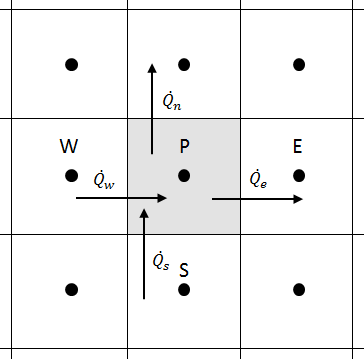
\includegraphics[scale=0.7]{FourMaterials/controlvolume2d}
	\caption{Heat fluxes through the faces of a control volume}
	\label{convol2d}
\end{figure}
The heat fluxes through the walls represented in figure \ref{convol2d} are defined by equation \ref{Fourier}. They are obtained integrating the expression in the vertical and horizontal directions.
\begin{equation}
\dot{Q}_{e}=-\int_{}^{S_{e}}\lambda\frac{\partial T}{\partial x}dS\approx-\left(\lambda\frac{\partial T}{\partial x}\right)_{e}S_{e}\approx-\lambda_{e}\frac{T_{E}-T_{P}}{d_{PE}}S_{e}
\end{equation}
\begin{equation}
\dot{Q}_{w}=-\int_{}^{S_{w}}\lambda\frac{\partial T}{\partial x}dS\approx-\left(\lambda\frac{\partial T}{\partial x}\right)_{w}S_{w}\approx-\lambda_{w}\frac{T_{P}-T_{W}}{d_{PW}}S_{w}
\end{equation}
\begin{equation}
\dot{Q}_{n}=-\int_{}^{S_{n}}\lambda\frac{\partial T}{\partial x}dS\approx-\left(\lambda\frac{\partial T}{\partial x}\right)_{n}S_{n}\approx-\lambda_{n}\frac{T_{N}-T_{P}}{d_{PN}}S_{n}
\end{equation}
\begin{equation}
\dot{Q}_{s}=-\int_{}^{S_{s}}\lambda\frac{\partial T}{\partial x}dS\approx-\left(\lambda\frac{\partial T}{\partial x}\right)_{s}S_{s}\approx-\lambda_{s}\frac{T_{P}-T_{S}}{d_{PS}}S_{s}
\end{equation}
where $T$ is the temperature at the given node, $d$ the distance between two nodes, and $\lambda$ the conductivity at the given face.

The inner heat of the material can be discretized as:
\begin{equation}
Q_{VP}=\int_{V_{P}}^{}\dot{q}_{v}dV\approx\dot{q}_{vP}V_{P}
\end{equation}

In the heat fluxes, though, the conductivity can have two different values: one on the left node and another one on the right node. Taking the value of the conductivity of just one node could lead to non-realistic results, because the heat fluxes evaluate the gradient of temperatures from one node to the other. To avoid this problem, the conductivity is determined using the harmonic mean \ref{harmonicmean}. This solution is justified operating the heat fluxes through the wall:
\begin{equation}
\dot{q}_{e}^{-}=\dot{q}_{e}^{+}
\end{equation}
\begin{equation}
-\lambda_{P}\frac{T_{e}-T_{P}}{d_{Pe}}=-\lambda_{E}\frac{T_{E}-T_{e}}{d_{Ee}}
\end{equation}
\begin{equation}
\dot{q}_{e}=-\lambda_{e}\frac{T_{E}-T_{P}}{d_{PE}}
\end{equation}
\begin{equation}
\lambda_{e}=\frac{d_{PE}}{\frac{d_{Pe}}{\lambda_{P}}+\frac{d_{Ee}}{\lambda_{E}}}
\label{harmonicmean}
\end{equation}

\subsection{Temporal discretization}
\label{TemporalDiscretizationConduction}
The time discretization is done using the First law of thermodynamics:
\begin{equation}
\int_{V_{P}}^{}\rho\frac{\partial u}{\partial t}dV=\sum\dot{Q}_{P}
\end{equation}
where $u$ is the internal energy of the control volume.
Assuming an incompressible material, the First law of thermodynamics is integrated over time. Taking $n$ as the previous instant of time and $n+1$ the instant of time that is going to be calculated:
\begin{equation}
\int_{t^{n}}^{t^{n+1}}\rho_{P}\frac{\partial\bar{u}_{P}}{\partial t}V_{P}dt=\int_{t^{n}}^{t^{n+1}}\sum\dot{Q}_{P}dt
\end{equation}
Rearranging the first term of the equation:
\begin{multline}
\int_{t^{n}}^{t^{n+1}}\rho_{P}\frac{\partial\bar{u}_{P}}{\partial t}V_{P}dt=\rho_{P}V_{P}\left(\bar{u}_{P}^{n+1}-\bar{u}_{P}^{n}\right)\approx \\
\rho_{P}V_{P}\left(u_{P}^{n+1}-u_{P}^{n}\right)=\rho_{P}V_{P}\bar{c}_{P}\left(T_{P}^{n+1}-T_{P}^{n}\right)
\end{multline}
To integrate the second term of the equation over time, a new variable $\beta$ is introduced, so as to be able to use an implicit, explicit or Crank-Nicholson scheme as explained in section \ref{TimeIntegration}.
\begin{equation}
\int_{t^{n}}^{t^{n+1}}\sum\dot{Q}_{P}dt=\left[\beta\sum\dot{Q}_{P}^{n+1}+\left(1-\beta\right)\sum\dot{Q}_{P}^{n}\right]\Delta t
\end{equation}

The discretized equation is finally obtained as the sum of both terms:
\begin{equation}
\rho_{P}V_{P}\bar{c}_{P}\frac{T_{P}^{n+1}-T_{P}^{n}}{\Delta t}=\beta\sum\dot{Q}_{P}^{n+1}+\left(1-\beta\right)\sum\dot{Q}_{P}^{n}
\end{equation}
where
\begin{multline}
	\dot{Q}_{P}=-\dot{Q}_{w}+\dot{Q}_{e}-\dot{Q}_{s}+\dot{Q}_{n}+\dot{q}_{vP}V_{P}= \\
	-\lambda_{w}\frac{T_{P}-T_{W}}{d_{PW}}S_{w}+\lambda_{e}\frac{T_{E}-T_{P}}{d_{PE}}S_{e}-\lambda_{s}\frac{T_{P}-T_{S}}{d_{PS}}S_{s}+\lambda_{n}\frac{T_{N}-T_{P}}{d_{PN}}S_{n}+\dot{q}_{vP}V_{P}
\end{multline}

\label{DiscrCond}
To simplify the equation, it can be rewritten with coefficients, dependant on the properties of the nearest nodes in the following form:
\begin{equation}
a_{P}T_{P}=a_{E}T_{E}+a_{W}T_{W}+a_{N}T_{N}+a_{S}T_{S}+b_{P}
\end{equation}
The coefficients are called discretization coefficients, and they are different for each node. The discretization coefficients are:
\begin{equation}
a_{E}=\beta\frac{\lambda_{e}S_{e}}{d_{PE}}
\end{equation}
\begin{equation}
a_{W}=\beta\frac{\lambda_{w}S_{w}}{d_{PW}}
\end{equation}
\begin{equation}
a_{N}=\beta\frac{\lambda_{n}S_{n}}{d_{PN}}
\end{equation}
\begin{equation}
a_{S}=\beta\frac{\lambda_{s}S_{s}}{d_{PS}}
\end{equation}
\begin{equation}
a_{P}=a_{E}+a_{W}+a_{N}+a_{S}+\rho_{P}V_{P}\bar{c}_{P}/\Delta t
\end{equation}
\begin{multline}
b_{P}=\frac{\rho_{P}V_{P}\bar{c}_{P}T_{P}^{n}}{\Delta t}+\beta\dot{q}_{vP}^{n+1}V_{P}+ \\
\left(1-\beta\right)\left[-\lambda_{w}\frac{T_{P}-T_{W}}{d_{PW}}S_{w}+\lambda_{e}\frac{T_{E}-T_{P}}{d_{PE}}S_{e}-\lambda_{s}\frac{T_{P}-T_{S}}{d_{PS}}S_{s}+\lambda_{n}\frac{T_{N}-T_{P}}{d_{PN}}S_{n}+\dot{q}_{vP}V_{P}\right]^{n}
\end{multline}

\section{Boundary conditions}
There are three kinds of boundary conditions that are common in conduction problems \cite{Bergman2011}:
\begin{itemize}
	\item Constant surface temperature: The temperature of a surface is prescribed. The condition is fulfilled just by substituting the value of the prescribed temperature in the conduction equation.
	\begin{equation}
	T_{wall}=T_{prescribed}
	\end{equation}
	\item Constant surface heat flux: The heat flux in a surface is prescribed. In some cases the surface is adiabatic, which means $\dot{q}=0$. In this case, the condition is imposed just by adding the heat flux to the conduction equation.
	\begin{equation}
	\dot{q}_{wall}=\dot{q}_{prescribed}
	\end{equation}
	\item Convection surface condition: This boundary condition refers to the existence of convection heat transfer at the surface. To fulfil this condition, it is necessary to calculate the heat transfer due to the convection:
	\begin{equation}
	\dot{q}_{conduction}=-\lambda\frac{T_{node}-T_{wall}}{d_{nw}}
	\end{equation}
	\begin{equation}
	\dot{q}_{convection}=\alpha\left(T_{g}-T_{wall}\right)
	\end{equation}
	\begin{equation}
	\dot{q}_{conduction}=\dot{q}_{convection}
	\end{equation}
	\begin{equation}
	\dot{q}=\frac{T_{g}-T_{node}}{\frac{1}{\alpha}+\frac{d_{nw}}{\lambda}}
	\end{equation}
	where $T_{g}$ is the temperature of the fluid next to the wall, $\alpha$ the convection heat transfer coefficient, $T_{node}$ the temperature of the node next to the wall, and $d_{nw}$ the distance from the node to the wall.
\end{itemize}